\section{Results}

The skewed data set contains 12244 datapoints each containing 784 dimensions of data. 
Review table~\ref{tab1} for the counts of the split dataset. 
The results of the MLP model and the CatB model are shown in Figures~\ref{fig1} and~\ref{fig2} respectively.
The same dataset was used for both models.

\begin{table}[htbp]
    \caption{Data set counts}\label{tab1}
    \begin{center}
        \begin{tabular}{c c c}
            \toprule            
            \textbf{Data}  & \textbf{\textit{Normal}}           & \textbf{\textit{Anomaly}} \\
            \textbf{Set}  & \textbf{\textit{0}}           & \textbf{\textit{1}} \\
            \midrule
            Training  & 9769 & 26 \\
            Test & 2441 & 8 \\
            \bottomrule           
        \end{tabular}
    \end{center}
\end{table}

After the models were fit to the data, the results were characterized. The first step in characterizing the results was to generate descriptive statistics.
The statistics for the MLP model are shown in Table~\ref{tab2} and the statistics for the CatB model are shown in Table~\ref{tab3}.

\begin{table}[htbp]
    \caption{MLP model descriptive statistics}\label{tab2}
    \begin{center}
        \begin{tabular}{c c c}
            \toprule            
            \textbf{Statistic}  & \textbf{\textit{Normal}}& \textbf{\textit{Anomaly}} \\
            \midrule
            Mean  & 0.0011367 & 0.516422\\
            Standard Deviation & 0.0326209 & 0.482698\\
            Minimum & 0.0000000 & 0.0000000 \\
            Maximum & 1.0000000 & 1.0000000\\
            \bottomrule
        \end{tabular}
    \end{center}
\end{table}

\begin{table}[htbp]
    \caption{CatB model descriptive statistics}\label{tab3}
    \begin{center}
        \begin{tabular}{c c c}
            \toprule            
            \textbf{Statistic}  & \textbf{\textit{Normal}} & \textbf{\textit{Anomaly}}\\
            \midrule
            Mean & 0.000452 & 0.365747 \\
            Standard Deviation & 0.004549 & 0.317829 \\
            Minimum &0.000000 & 0.000976 \\
            Maximum &0.160315& 0.782518 \\
            \bottomrule
        \end{tabular}
    \end{center}
\end{table}
        

\begin{figure}[htbp]
    \centerline{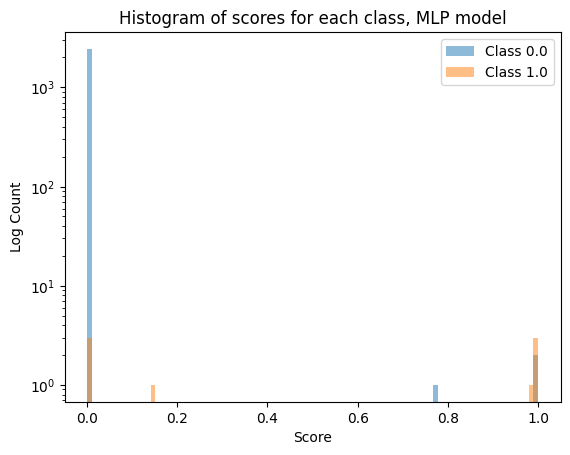
\includegraphics[width=0.5\textwidth]{resources/ch3/fig1.png}}
    \caption{Multi-layer perception model results.}\label{fig1}
\end{figure}


\begin{figure}[htbp]
    \centerline{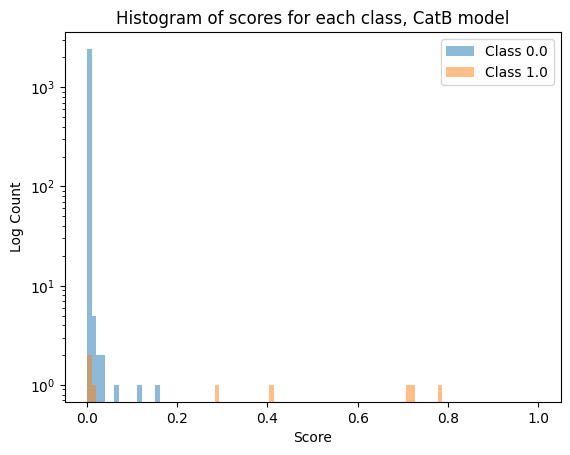
\includegraphics[width=0.5\textwidth]{resources/ch3/fig2.png}}
    \caption{CatBoost model results.}\label{fig2}
\end{figure}


After reviewing the descriptive statistics and the histogram plots of the results there appears to be a seperation between the anomalous data and the normal data.
To further characterize the results, confusion matrices were generated for the MLP model and the CatB model. The confusion matrices are shown in Table~\ref{tab4} and Table~\ref{tab5} respectively.
Also, the accuracy of the models were calculated. Due to the large number of non-anomalous data points, the accuracy is not a good measure of the model's performance.
A better measure of the model's performance is the precision and recall\ \cite{precision_recall_wiki}. The precision and recall for each model with varying thresholds are shown with their confusion matrix data.

\begin{table}[htbp]
    \caption{MLP model confusion matrix}\label{tab4}
    \begin{center}
        \begin{tabular}{c|cc|cc|cc|cc}
            \toprule 
                & $0.5\sigma$& &  $1.0\sigma$ & & $2.0\sigma$ & & $3.0\sigma$\\           
            \textbf{Predicted}  & \textbf{\textit{N}} & \textbf{\textit{A}}& \textbf{\textit{N}} & \textbf{\textit{A}}& \textbf{\textit{N}} & \textbf{\textit{A}}& \textbf{\textit{N}} & \textbf{\textit{A}}\\
            \midrule
            Actual Normal & 2438 & 3 & 2438 & 3& 2438 & 3& 2438 & 3\\
            Actual Anomaly & 3 & 5 & 3 & 5& 3 & 5& 3 & 5\\
            \midrule
            Accuracy & 0.9975 & & 0.9975 & & 0.9975 & & 0.9975 & \\
            Threshold & 0.0175 & & 0.0338 & & 0.0664 & & 0.0990 & \\
            Precision & 0.625 & & 0.625 & & 0.625 & & 0.625 & \\
            Recall & 0.625 & & 0.625 & & 0.625 & & 0.625 & \\
            \bottomrule
        \end{tabular}
    \end{center}
\end{table}

\begin{table}[htbp]
    \caption{CatB model confusion matrix}\label{tab5}
    \begin{center}
        \begin{tabular}{c|cc|cc|cc|cc}
            \toprule 
                & $0.5\sigma$& &  $1.0\sigma$ & & $2.0\sigma$ & & $3.0\sigma$\\           
            \textbf{Predicted}  & \textbf{\textit{N}} & \textbf{\textit{A}}& \textbf{\textit{N}} & \textbf{\textit{A}}& \textbf{\textit{N}} & \textbf{\textit{A}}& \textbf{\textit{N}} & \textbf{\textit{A}}\\
            \midrule
            Actual Normal & 2394 & 47 & 2415 & 26 & 2428 & 13 & 2431 & 10\\
            Actual Anomaly & 1 & 7 & 1 & 7& 2 & 6 & 2 & 6\\
            \midrule
            Accuracy & 0.9804 & & 0.9890 & & 0.9938 & & 0.9951 & \\
            Threshold & 0.0027 & & 0.0050 & & 0.0096 & & 0.0141 & \\
            Precision & 0.130 & & 0.212 & & 0.316 & & 0.375 & \\
            Recall & 0.875 & & 0.875 & & 0.750 & & 0.750 & \\
            \bottomrule
        \end{tabular}
    \end{center}
\end{table}


\section{Conclusion}

Assignment 5 was a time consuming task due to the installation issues with ADBench. The authors did not document the versions of the libraries they used during their paper.
Withstanding the installation issues, the results of the MLP model and the CatB model show that the models are able to distinguish between the normal data and the anomalous data.
However, the precision and recall of these simple and untuned models are not ideal. This was a good excercise in understanding anomaly detection in general and the capabilities compiled by the Authors within ADBench.







